\section{9. Производные высших порядков. Формула Лейбница для $n$--ой производной произведения функций. Формула Тейлора с остаточным членом в форме Пеано. Разложения функций $e^{x}$, $\sin x$, $\cos x$, $\ln(1+x)$ и $(1+x)^{\alpha}$. Достаточное условия локального экстремума в терминах высших производных. Формула Тейлора с остаточным членом в форме Лагранжа. Выпуклые функции. Дифференциальные условия выпуклости. Неравенство Йенсена.}

    Производные высших порядков определяются индуктивно.
    
    \begin{definition}
        Пусть $n \in \N$. Положим $f^{(1)} = f'$.
        Если $n > 1$, функция $f^{(n-1)}$ определена в некоторой окрестности точки $a$
        и дифференцируема в самой точке $a$, то функция $f$ называется
        \textit{дифференцируемой n раз} в точке $a$, и ее производная $n$-ого порядка
        в точке $a$ определяется равенством $f^{(n)}(a) = (f^{(n-1)})'(a)$.
        Считаем также $f^{(0)} = f$.    
    \end{definition}
    
    Функция $f$ называется $n$ раз дифференцируемой на множестве $E$,
    если она $n$ раз дифференцируема в каждой точке из $E$. 
    
    \begin{note}
        Если $n > 1$, то существование производной $n$-ого порядка в точке $a$
        влечет существование производных $n-1$-ого порядка в некоторой окрестности точки $a$.
    \end{note}
    
    Ввиду линейности дифференцирования, по индукции устанавливается, что $(\alpha f + \beta g)^{(n)} = \alpha f^{(n)} + \beta g^{(n)}$, если $\exists f^{(n)}, g^{(n)}$.
    Для произведения справедлива следующая формула.
    
    \begin{theorem}{Формула Лейбница.}\\
        Если $f$ и $g$ дифференцируемы $n$ раз в точке $x$,
        то в точке $x$ также дифференцируема $n$ раз функция $f \cdot g$,
        причем справедлива формула: \[(f\cdot g)^{(n)} (x) = \sum_{k = 0}^{n} C_{n}^{k}f^{(k)}(x)g^{(n-k)}(x)\]
    \end{theorem}
    
    \begin{proof}
        Докажем индукцией по $n$. При $n = 1$ равенство известно $(fg)'(x) = f'(x)g(x) + f(x)g'(x)$.
        Предположим, утверждение верно для $n$, тогда (опуская аргумент $x$)
        \[(fg)^{(n+1)} = ((fg)^{n})' = \]
        \[= (\sum_{k = 0}^{n} C_{n}^{k}f^{(k)}(x)g^{(n-k)}(x))' = \]
        \[= \sum_{k = 0}^{n} C_{n}^{k}f^{(k+1)}(x)g^{(n-k)}(x) + \sum_{k = 0}^{n} C_{n}^{k}f^{(k)}(x)g^{(n-k+1)}(x) = \]
        \[= f^{(n+1)}g + \sum_{k = 1}^{n} C_{n}^{k-1}f^{(k)}(x)g^{(n+1-k)}(x) + \sum_{k = 1}^{n} C_{n}^{k}f^{(k)}(x)g^{(n+1-k)}(x) + fg^{(n+1)} = \]
        \[= \sum_{k = 1}^{n} (C_{n}^{k-1} + C_{n}^{k})f^{(k)}(x)g^{(n+1-k)}(x) + f^{(n+1)}g + fg^{(n+1)} =
        \sum_{k = 0}^{n+1} C_{n+1}^{k}f^{(k)}(x)g^{(n+1-k)}(x) \]
        Так как $C_{n}^{k-1} + C_{n}^{k} = C_{n+1}^{k}$.
    \end{proof}
    
    \begin{definition}
        Пусть $n \in \N$ и функция $f$ дифференцируема $n$ раз в точке $a$.
        Тогда равенство:
        \[f(x) = \sum_{k = 0}^{n} \frac{f^{(k)}(a)}{k!}(x-a)^k + r_n(x)\]
        называется \textit{формулой Тейлора} порядка $n$ функции $f$ в точке $a$.\\
        При этом многочлен $P_n(x) = P_{n, a, f}(x) = \sum_{k = 0}^{n} \frac{f^{(k)}(a)}{k!}(x-a)^k$
        называется \textit{многочленом Тейлора},
        $r_n(x) = r_{n, a, f}(x)$ - \textit{остаточным членом}.
    \end{definition}
    
    \begin{theorem}{Остаточный член в форме Пеано.}\\
        Пусть $n \in \N$ и функция $f$ дифференцируема $n$ раз в точке $a$.
        Тогда \[f(x) = \sum_{k = 0}^{n} \frac{f^{(k)}(a)}{k!}(x-a)^k + o((x-a)^n), \ x \to a\]
        то есть $r_n(x) = o((x-a)^n)$ при $x \to a$.
    \end{theorem}
    
    \begin{proof}
        Пусть $P_n(x) = \sum_{k = 0}^n \frac{f^{(k)}(a)}{k!}(x-a)^k$,
        тогда $P^{(k)}(a) = f^{(k)}(a), \ 0 \leq k \leq n$.
        Поэтому для остаточного члена $r_n(x) = f(x) - P_n(x)$
        выполнено $r_n(a) = r_n'(a) = \dots = r_n^{(n)}(a) = 0$.
        По правилу Лопиталя
        \[\lim_{x \to a} \frac{r_n(x)}{(x-a)^n} = \lim_{x \to a} \frac{r_n'(x)}{n(x-a)^{n-1}} = \dots = \lim_{x \to a} \frac{r_n^{(n-1)}(x)}{n!(x-a)}\]
        Последний предел существует по определению $n$-й производной в точке $a$:
        \[\lim_{x \to a} \frac{r_n^{(n-1)}(x)}{n!(x-a)} = \frac{1}{n!}\lim_{x \to a} \frac{r_n^{(n-1)}(x) - r_n^{(n-1)}(a)}{(x-a)} = \frac{r_n^{(n)}(a)}{n!} = 0\]
        следовательно, $r_n(x) = o((x-a)^n)$ при $x \to a$.
    \end{proof}
    
    \begin{corollary}{Достаточное условие локального экстремума.}\\
        Пусть $n \in \N$, функция f дифференцируема $n$ раз в точке $a$ и $f'(a) = \dots = f^{(n-1)}(a) = 0$,
        но $f^{(n)}(a) \neq 0$. Тогда
        \begin{enumerate}
            \item если $n$ четно и $f^{(n)}(a) < 0$ ($f^{(n)}(a) > 0$), то $a$ является точкой
            строгого локального максимума (минимума) функции $f$.
            \item если $n$ нечетно, то $a$ не является точкой локального
            экстремума функции $f$.
        \end{enumerate}
    \end{corollary}
    
    \begin{proof}
        По предыдущей теореме
        \[f(x) - f(a) = \frac{f^{(n)}(a)}{n!}(x-a)^n + o((x-a)^n) =\]
        \[= (\frac{f^{(n)}(a)}{n!} + \alpha(x))\cdot (x-a)^n\]
        где $\alpha(x) \to 0$ при $x \to a$. Найдется такое $\delta > 0$,
        что $|\alpha(x)| < |\frac{f^{(n)}(a)}{n!}| \ \forall x \in \mathring{B}_{\delta}(a)$,
        поэтому $sign(\frac{f^{(n)}(a)}{n!} + \alpha(x)) = sign(f^{(n)}(a)) \ \forall x \in \mathring{B}_{\delta}(a)$,
        и значит, в $\mathring{B}_{\delta}(a)$ $\ sign(f(x) - f(a)) = sign(f^{(n)}(a)(x-a)^n)$.\\
        Что в 1 случае дает одинаковые знаки при $x < a$ и $x > a$. И во втором - разные.
    \end{proof}
    
    \begin{theorem}{О единственности разложения.}\\
        Пусть $p_{1}(x), p_{2}(x)$ -- такие многочлены степени $\leq n$, что $f(x) - p_{1}(x) = o((x-a)^{n})$
        и $f(x) - p_{2}(x) = o((x-a)^{n}), x \to a$. Тогда $p_{1}(x) = p_{2}(x)$.
    \end{theorem}
    
    \begin{proof}
        Положим $q(x) = p_{1}(x) - p_{2}(x)$, тогда $q(x) = o((x-a)^{n})$. Покажем, что $q(x)$ -- нулевой многочлен.\\
        Пусть $q(x) = c_{0} + c_{1}(x-a) + ... + c_{n}(x-a)^{n}$. Предположим, что $\exists c_{i} \neq 0$. Тогда положим $j = \min\{k: c_{k} \neq 0\}$. Поделим равенство на $(x-a)^{j}$ получим $q(x) = o((x-a)^{n-j})$. Перейдем к пределу при $x \to a$, тогда $c_{j} = 0$. Противоречие.
    \end{proof}
    
    \begin{theorem}{Основные разложения.}\\
        $1)$ Если $f(x) = e^{x}$, то $f^{(k)}(0) = e^{0} = 1, k \in \N$. Следовательно, 
        \[e^{x} = \sum_{k=0}^{n}\frac{x^{k}}{k!} + o(x^{n}), x \to 0\]
        $2)$ Если $f(x) = \sin(x)$. Тогда (по индукции) $f^{(n)}(x) = \sin(x + \frac{\pi}{2}n), n \in \N$. Поэтому $f^{(2k)}(0) = 0, f^{(2k+1)}(0) = (-1)^{k}$. Следовательно, 
        \[\sin(x) = \sum_{k = 0}^{n} \frac{(-1)^{k} x^{2k+1}}{(2k+1)!} + o(x^{2n+2}), x \to 0\]
        $3)$ Если $f(x) = \cos(x)$. Тогда (по индукции) $f^{(n)}(x) = \cos(x + \frac{\pi}{2}n), n \in \N$. Поэтому $f^{(2k)}(0) = (-1)^{k}, f^{(2k + 1)}(0) = 0$. Следовательно, 
        \[\cos(x) = \sum_{k = 0}^{n} \frac{(-1)^{k} x^{2k}}{(2k)!} + o(x^{2n+1}), x \to 0\]
        $4)$ Если $f(x) = (1+x)^{\alpha}, \alpha \in \R$, то $f^{(k)}(x) = \alpha \cdot (\alpha - 1) \cdot ... \cdot (\alpha - k + 1)(1+x)^{\alpha - k}$. \\
        Положим $c_{\alpha}^{0} = 1, c_{\alpha}^{k} = \frac{\alpha \cdot (\alpha - 1) \cdot ... \cdot (\alpha - k + 1)}{k!}$. Следовательно, 
        \[(1+x)^{\alpha} = \sum_{k = 0}^{n} c_{\alpha}^{k}x^{k} + o(x^{n}), x \to 0\]
        В частности $\frac{1}{1+x} = \sum_{k = 0}^{n} (-1)^{k} x^{k} + o(x^{n}), x \to 0$. \\
        $5)$ Если $f(x) = \ln(1+x)$, то $f(0) = 0$, $f^{(k)}(x) = \frac{(-1)^{k-1}(k-1)!}{(1+x)^{k}}$. Следовательно,
        \[\ln(1+x) = \sum_{k = 1}^{n} \frac{(-1)^{k-1}}{k}x^{k} + o(x^{n}), x \to 0\]
    \end{theorem}
    
    \begin{theorem}{Остаточный член в форме Лагранжа.}\\
        Пусть функция $f$ дифференцируема $n+1$ раз на $(\alpha , \beta)$ и $a \in (\alpha, \beta)$. Тогда для любой точки $x \in (\alpha, \beta),\ x \neq a$, найдется точка $c$, лежащая между $a$ и $x$, что
        \[f(x) = \sum_{k = 0}^{n}\frac{f^{(k)}(a)}{k!}(x-a)^{k} + \frac{f^{(n+1)}(c)}{(n+1)!}(x-a)^{n+1}\]
        т.е. $r_{n}(x) = \frac{f^{(n+1)}(c)}{(n+1)!}(x-a)^{n+1}$.
    \end{theorem}
    
    \begin{proof}
        Пусть для определенности $x > a$. Рассмотрим функции $\phi (t) = f(t) + f'(t)(x-t) + ... + \frac{f^{(n)}(t)}{n!}(x-t)^{n}$, $\psi (t) = (x-t)^{n+1}$. Функции $\phi$ и $\psi$ дифференцируемы на $[a,x]$, $\phi'(t) = \frac{f^{(n+1)}(t)}{n!}(x - t)^{n}$ и $\psi'(t) = -(n+1)(x-t)^{n}$, причем $\psi' \neq 0$ на $(a, x)$. Тогда по теореме Коши найдется такая точка $c \in (a,x)$, что
        \[\frac{\phi(x) - \phi(a)}{\psi(x) - \psi(a)} = \frac{\phi'(c)}{\psi'(c)} \lra \frac{f(x) - \sum\limits_{k=0}^{n}\frac{f^{(k)}(a)}{k!}(x-a)^{k}}{-(x-a)^{n+1}} = \frac{\frac{f^{(n+1)}(c)}{n!}(x - c)^{n}}{-(n+1)(x-c)^{n}},\]
        откуда получаем, что $r_{n}(x) = \frac{f^{(n+1)(c)}}{(n+1)!}(x-a)^{n+1}$.
    \end{proof}
    
    \begin{definition}
        Пусть $f$ определена на промежутке $I$. Функция $f$ называется \textit{выпуклой} (или выпуклой вниз) на $I$, если для любых $x_{1}, x_{2} \in I, x_{1} \neq x_{2}$ и $t \in (0,1)$ выполнено
        \[f((1-t)x_{1} + tx_{2}) \leq (1-t)f(x_{1}) + tf(x_{2}).\]
        Если неравенство строгое, то говорят, что $f$ \textit{строго выпукла} на $I$. Функция $f$ называется \textit{вогнутой}(или выпуклой вверх) на $I$, если функция $(-f)$ выпукла на $I$. Аналогично определяется строгая вогнутость.
    \end{definition}
    
    \begin{note}
        Геометрический смысл.\\
        Выпуклость означает, что график функции лежит \textit{не выше} любой своей хорды.
        \begin{center}
            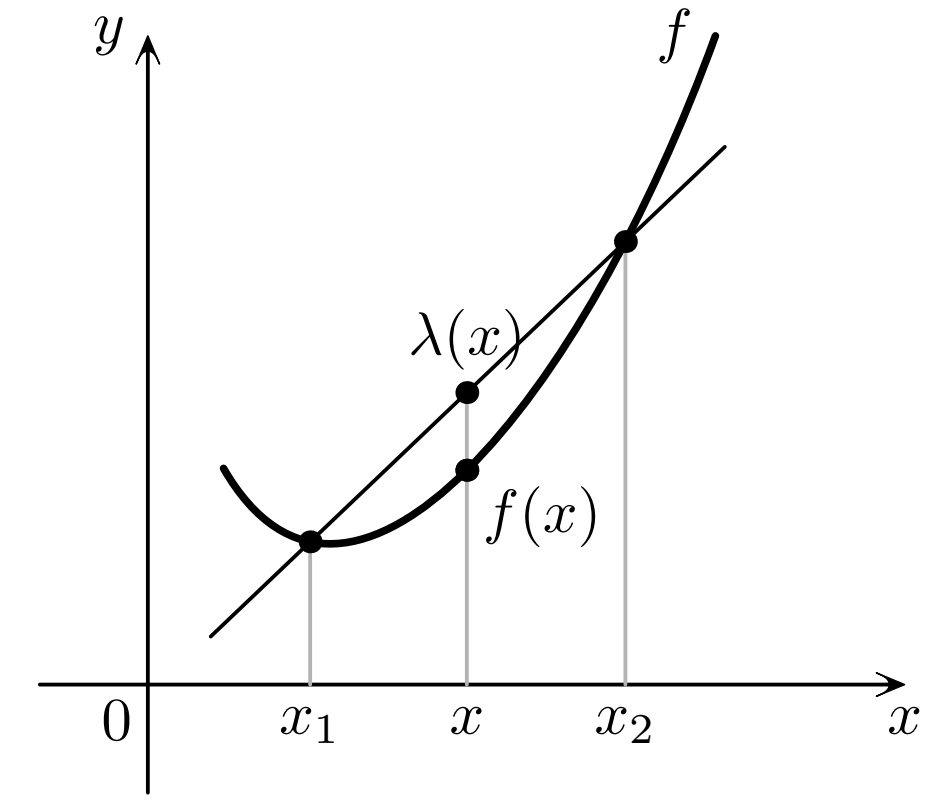
\includegraphics[width=0.35\textwidth]{ex2.png}
        \end{center}
    \end{note}
    
    Проверка выпуклости по определению не всегда удобна. Однако, если функция дифференцируема, то такая проверка легко описывается.
    
    \begin{theorem}
        Пусть функция $f$ непрерывна на промежутке $I$ и дифференцируема на $int(I)$. Тогда следующие утверждения эквивалентны:
        \begin{enumerate}
            \item $f$ выпукла на $I$;
            \hypertarget{sec_punkt}{\item} $f(x) \geq f(x_{0}) + f'(x_{0})(x-x_{0})$ для всех $x \in I$ и $x_{0} \in int(I)$;
            \item $f'$ возрастает на $int(I)$;
        \end{enumerate}
    \end{theorem}
    
    \begin{proof}
        $(1 \Rightarrow 2)$. Пусть $x \in I, x_{0} \in int(I).$ Пусть $h = x - x_{0}$ и $t \in (0,1)$. По определению выпуклости $f(x_{0} + th) \leq (1-t)f(x_{0}) + tf(x_{0} + h)$. Это неравенство можно переписать в виде
        \[f(x_{0} + th) - f(x_{0}) \leq t(f(x_{0} + h) - f(x_{0})),\]
        откуда, пользуясь дифференцируемостью $f$ в точке $x_{0}$, имеем
        \[tf'(x_{0})h + o(th) \leq t(f(x_{0} + h) - f(x_{0})), t \to 0.\]
        Поделим обе части на $t$ и перейдем к пределу при $t \to 0$. Тогда 
        \[f'(x_{0})h \leq f(x_{0} + h) - f(x_{0}).\]
        $(2 \Rightarrow 3)$. Для $x,y \in int(I)$ имеем
        \[f(y) - f(x) \geq f'(x)(y-x) \Rightarrow f(x) - f(y) \leq -f'(x)(y-x).\]
        \[f(x) - f(y) \geq f'(y)(x-y) \Rightarrow f(y) - f(x) \leq -f'(y)(y-x).\]
        Складывая неравенства, получим $(f'(y) - f'(x))(y-x) \geq 0$.\\
        $(3 \Rightarrow 1)$. Пусть $x_{1}, x_{2} \in I, x_{1} < x_{2}$ и $t \in (0,1)$. Положим $x = (1-t)x_{1} + tx_{2}$.\\
        По теореме Лагранжа $f(x) - f(x_{1}) = f'(c_{1})(x-x_{1})$ и $f(x_{2}) - f(x) = f'(c_{2})(x_{2} - x)$ для некоторых $c_{1} \in (x_{1}, x)$ и $c_{2} \in (x, x_{2})$. В силу возрастания производной $f'(c_{1}) \leq f'(c_{2})$ и, значит,
        \[\frac{f(x) - f(x_{1})}{x - x_{1}} \leq \frac{f(x_{2}) - f(x)}{x_{2} - x}.\]
        Так как $x - x_{1} = t(x_{2} - x_{1})$ и $x_{2} - x = (1-t)(x_{2} - x_{1})$, то последнее неравенство равносильно $\frac{f(x) - f(x_{1})}{t} \leq \frac{f(x_{2}) - f(x)}{1 - t}$ или $f(x) \leq (1-t)f(x_{1}) + tf(x_{2})$. Следовательно, $f$ выпукла на $I$.
    \end{proof}
    
    \begin{note}
        Геометрический смысл \hyperlink{sec_punkt}{пункта 2} означает, что график выпуклой функции лежит не ниже всякой своей касательной.
    \end{note}
    
    \begin{corollary}
        Пусть функция $f$ непрерывна на промежутке $I$ и дважды дифференцируема на $int(I)$.
        \begin{enumerate}
            \item Функция $f$ выпукла на $I$ тогда и только тогда, когда $f'' \geq 0$ на $int(I)$.
            \item Если $f'' > 0$ на $I$, то функция $f$ строго выпукла на $int(I)$.
        \end{enumerate}
    \end{corollary}
    
    \begin{theorem}{Неравенство Йенсена.} \\
        Пусть $f$ выпукла на $I$, $x_1, x_2, \dots, x_n \in I$,
        $\lambda_1, \lambda_2, \dots, \lambda_n \geq 0$ и $\lambda_1 + \lambda_2 + \dots + \lambda_n = 1$.
        Тогда $f(\lambda_1\cdot x_1 + \lambda_2\cdot x_2 + \dots + \lambda_n\cdot x_n) \leq \lambda_1\cdot f(x_1) + \lambda_2\cdot f(x_2) + \dots + \lambda_n\cdot f(x_n)$.
    \end{theorem}
    
    \begin{proof}
        ММИ по $n$. При $n = 2$ -- определение выпуклости.
        Пусть утверждение верно для $n$.
        Тогда $f(\lambda_1\cdot x_1 + \lambda_2\cdot x_2 + \dots + \lambda_n\cdot x_n + \lambda_{n+1}\cdot x_{n+1}) \leq (1-\lambda_{n+1})f(y) + \lambda_{n+1}f(x_{n+1})$.
        \[y = \frac{\lambda_1}{1 - \lambda_{n+1}}x_1 + \dots + \frac{\lambda_n}{1 - \lambda_{n+1}}x_n\]
        При этом справедливо неравенство: $\frac{\lambda_1}{1 - \lambda_{n+1}} + \dots + \frac{\lambda_n}{1 - \lambda_{n+1}} = 1$. Тогда
        \[f(y) = f(\frac{\lambda_1}{1 - \lambda_{n+1}}x_1 + \dots + \frac{\lambda_n}{1 - \lambda_{n+1}}x_n) \leq \]
        \[\leq \frac{\lambda_1}{1 - \lambda_{n+1}}f(x_1) + \dots + \frac{\lambda_n}{1 - \lambda_{n+1}}\cdot f(x_n)\]
        \[\Rightarrow f(\lambda_1\cdot x_1 + \lambda_2\cdot x_2 + \dots + \lambda_n\cdot x_n + \lambda_{n+1}\cdot x_{n+1}) \leq\]
        \[\leq (1-\lambda_{n+1})(\frac{\lambda_1}{1 - \lambda_{n+1}}f(x_1) + \dots + \frac{\lambda_n}{1 - \lambda_{n+1}}\cdot f(x_n)) + \lambda_{n+1}f(x_{n+1}) =\]
        \[= \lambda_1\cdot f(x_1) + \lambda_2\cdot f(x_2) + \dots + \lambda_n\cdot f(x_n)\]
    \end{proof}